\documentclass[11pt, 
				t, 
				beamer,
				%trans,
				%handout,
				breaklinks = true,
				bookmarksnumbered,
				spanish,
				]{beamer}


%% Opciones:
%%    - beamer:  Para crear la presentación. Crea solapas y transiciones.
%%    - trans:   No crea solapas (overlays). Versión para imprimir en transparencia
%%               por si falla el cañón de proyección, o el ordenador.
%%    - handout: Versión para imprimir y repartir entre los oyentes.
%%    - draft:   compilación más rápida mientras se trabaja (no incluye imágenes).
%%
%%    - t: Alineación del contenido de las transparencias: b(ottom), c(enter), t(op).  
%%
%%    - 11pt: Es el tamaño de letra que utiliza Beamer.
%%            Lo puedes cambiar a: 8pt, 9pt, 10pt (smaller), 12pt (bigger) y más...


%----------------------------------------------------------------------------
%% Paquetes generales necesarios

%\usepackage[latin1]{inputenc}
\usepackage[spanish]{babel}
\usepackage{mathtools}  % Comandos ampliados en el entorno matemático
\usepackage{graphicx}

\usepackage[
	url = false,
	style = authoryear,
	bibstyle = authoryear,
	hyperref = true,
%	backref = true,
	backend = bibtex,
	]{biblatex}

\bibliography{referencias}


%----------------------------------------------------------------------------
%% Información de la portada y de los marcos exteriores


\title [Presentacion de la asignatura. Normativa
	(\insertframenumber/\inserttotalframenumber)
	]
	{\Large\bf Automatización de máquinas y procesos\\ Curso 2014-2015}

\author[José V. Salcedo]{}

\date{}

\institute[Departamento de Ingeniería de Sistemas y Automática]{}

%----------------------------------------------------------------------------
%% Configuración de la versión para imprimir:
%%    - handout: para imprimir en papel y repartir entre los oyentes
%%    - trans: para imprimir transparencias

\usepackage{pgfpages}

\mode<handout>{
	\usepackage[a4, dvips, landscape, off]{crop}
	\pgfpagesuselayout{4 on 1}[a4paper, border shrink=5mm, landscape]
	\usetheme{Montpellier}
	\usecolortheme{dove}
	}

\mode<trans>{
	\usepackage[a4, dvips, landscape, off]{crop}
	\pgfpagesuselayout{resize to}[a4paper, border shrink=5mm, landscape]
	}


%----------------------------------------------------------------------------
%----------------------------------------------------------------------------
%----------------------------------------------------------------------------

% Para conseguir el efecto de semitransparencia para las pausas en los ítems
\setbeamercovered{dynamic}

%----------------------------------------------------------------------------
%----------------------------------------------------------------------------
%----------------------------------------------------------------------------

%% Puedes cambiar el aspecto eligiendo un tema o plantilla de presentación
%% que incluye la configuración de todos los elementos de la presentación:
%%     - Interiores: el contenido de las transparencias
%%     - Exteriores: los marcos informativos y barras de navegación
%%     - Colores: la paleta de colores de las transparencias
%%     - Tipos de letra

%----------------------------------------------------------------------------
%% Elección de un tema completo

%\mode<beamer>{\usetheme{Warsaw}} % Usa este tema en el modo presentación
\mode<beamer>{\usetheme[compress]{Berlin}} % Usa este tema en el modo presentación
\mode<trans>{\usetheme[compress]{Szeged}}  % Usa este tema en el modo transparencias

% ------------------------------
%% Temas sin barra de navegación.
%% Por favor, revisa el manual de usuario de BEAMER.

%\usetheme{default} 
%\usetheme{Bergen} 
%\usetheme{Boadilla} 
%\usetheme{Madrid} 
%\usetheme{AnnArbor}
%\usetheme{CambridgeUS}
%\usetheme{Pittsburgh}
%\usetheme{Rochester}

% ------------------------------
%% Temas con barra de navegación tipo árbol.
%% Por favor, revisa el manual de usuario de BEAMER.

%\usetheme{Antibes}
%\usetheme{JuanLesPins}
%\usetheme{Montpellier}

% ------------------------------
%% Temas con barra de navegación lateral.
%% Por favor, revisa el manual de usuario de BEAMER.

%\usetheme[]{Berkeley}
%\usetheme[]{PaloAlto}
%\usetheme[]{Goettingen}
%\usetheme[]{Marburg}
%\usetheme[]{Hannover}

% ------------------------------
%% Temas con un pequeño marco de navegación.
%% Marca el transcurso de la presentación con circulitos.
%% Por favor, revisa el manual de usuario de BEAMER.

%\usetheme[compress]{Berlin}
%\usetheme[compress]{Ilmenau} % Variación de Berlin
%\usetheme[compress]{Dresden}
%\usetheme[compress]{Darmstadt}
%\usetheme[compress]{Frankfurt}
%\usetheme[compress]{Singapore}
%\usetheme[compress]{Szeged}

% ------------------------------
%% Temas con una tabla de contenido en la parte superior.
%% Incluye secciones y subsecciones.
%% Por favor, revisa el manual de usuario de BEAMER.

%\usetheme{Copenhagen}
%\usetheme{Luebeck}
%\usetheme{Malmoe}
%\usetheme{Warsaw}

%----------------------------------------------------------------------------
%% Puedes cambiar el aspecto interior de un tema, el contenido de cada diapositiva.
%% Por favor, revisa el manual de usuario de BEAMER.

%\useinnertheme{default}
%\useinnertheme{circles}
%\useinnertheme{rectangles}
%\useinnertheme[shadow=false]{rounded}
%\useinnertheme{inmargin}

%----------------------------------------------------------------------------
%% Puedes cambiar el aspecto exterior de un tema, los marcos exteriores.
%% Por favor, revisa el manual de usuario de BEAMER.

%\useoutertheme{default}
%\useoutertheme{infolines}
%\useoutertheme{miniframes}
%\useoutertheme{smoothbars}
%\useoutertheme{sidebar}
%\useoutertheme[]{split}
%\useoutertheme[]{shadow}
%\useoutertheme{tree}
%\useoutertheme{smoothtree}

%----------------------------------------------------------------------------
%% Puedes cambiar todos los colores utilizados en un tema.
%% Por favor, revisa el manual de usuario de BEAMER.

%\usecolortheme[]{structure}
%\usecolortheme{sidebartab}
%\usecolortheme[overlystylish]{albatross}
%\usecolortheme{beetle}
%\usecolortheme{crane}
%\usecolortheme{dove}
%\usecolortheme{fly}
%\usecolortheme{seagull}
%\usecolortheme{wolverine}
%\usecolortheme{beaver}
%----------------------------------------------------------------------------
%% Puedes cambiar sólo los colores interiores
%% Por favor, revisa el manual de usuario de BEAMER.

%\usecolortheme{lily}
%\usecolortheme{orchid} 
%\usecolortheme{rose} 

%----------------------------------------------------------------------------
%% Puedes cambiar sólo los colores exteriores.
%% Por favor, revisa el manual de usuario de BEAMER.

%\usecolortheme{whale} 
%\usecolortheme{seahorse} 
%\usecolortheme{dolphin} 

%----------------------------------------------------------------------------
%% Puedes cambiar los tipos de letra utilizados en un tema.
%% Por favor, revisa el manual de usuario de BEAMER.

\usefonttheme{professionalfonts} % Para que las ecuaciones tengan mejor aspecto
%\usefonttheme[]{serif}
%\usefonttheme[]{structurebold}

%% Y también puedes elegir un tipo de letra cargando culquiera de los siguientes paquetes:
%% avant, bookman, chancery, charter, euler, helvet, mathtime, 
%% mathptm, mathptmx, newcent, palatino, pifont, utopia.

%\usepackage{avant}

%----------------------------------------------------------------------------
%----------------------------------------------------------------------------
%----------------------------------------------------------------------------


%Antes de cada sección incluye la tabla de contenidos destacando la actual

\AtBeginSection[]
	{
   \begin{frame}
       \frametitle{Resumen}
       \tableofcontents[currentsection]
   \end{frame}
	}


\begin{document}

% Citas bibliográficas

\nocite{moreno1999automatizacion}
\nocite{moreno1999grafcet}
\nocite{piedrafita2004ingenieria}
\nocite{ramirez1994automatizacion}

%--------------------------------------

%\begin{frame}[fragile, plain, label = portada]

\titlepage

\begin{center}

\vspace*{-2cm}

\textcolor{red}{\Large\bf Presentación de la asignatura. Normativa}\\[2ex]

\scriptsize
\begin{tabular}{ c c c c}
José V. Salcedo \\
\href{mailto:jsalcedo@upv.es}{\textcolor{green}{\footnotesize\texttt{jsalcedo@upv.es}}}
\end{tabular}

\vspace*{1.0cm}


\includegraphics[
	height = 1cm
	]{etsid_color}
\hspace*{5.5cm}

\includegraphics[
	height = 1.2cm
	]{isa}
\end{center}
\end{frame}

% Tabla de contenidos

\begin{frame}[fragile, label = indice]
\frametitle{Resumen}
\tableofcontents[pausesections]
\end{frame}

% Contenidos

\section{Profesor}

\begin{frame}[fragile, label = profesorado]
\frametitle{Profesor}
\begin{itemize}
    \item Jairo Sacoto
    \begin{itemize}
        \item Departamento de Ingeniería de Sistemas y Atomática
        \item{Tutorías: bajo demanda al correo \href{mailto:jsacoto@isa.upv.es}{\textcolor{red}{jsacoto@upv.es}}}
        \item Despacho: 2ª planta edificio 5C (\href{http://www.upv.es/plano/plano-2d-es.html?entidad=ACOM}{\textcolor{red}{Plano interactivo}} de la UPV)
    \end{itemize}
\end{itemize}


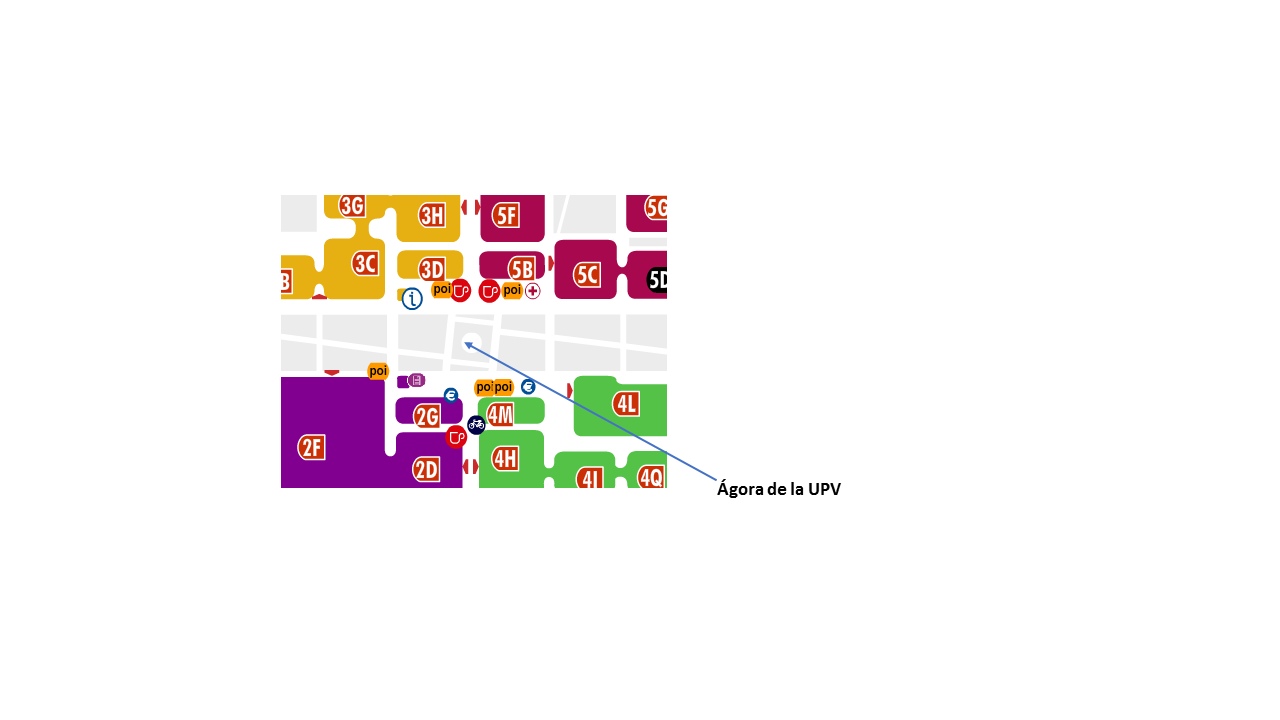
\includegraphics[trim=5cm 0cm 5cm 5cm, clip, width=1.2\textwidth]{PlanoUPV}

\end{frame}


\section{¿Qué estudia la asignatura?}

\begin{frame}[t,fragile, label=sistemas]
\frametitle{Automatización}

\begin{itemize}
\item La automatización es la ciencia que se encarga de diseñar aquellos dispositivos que permiten hacer funcionar de manera autónoma máquinas y procesos

\item En la asignatura \textbf{Electrónica y automática} se han diseñado dispositivos de control para procesos continuos

\item En concreto se han diseñado reguladores o controladores de tipo PID

\item En esta asignatura se van a diseñar dispositivos de control para procesos de eventos discretos
\end{itemize}
   
\end{frame}


\section{Objetivos básicos}

\begin{frame}[fragile, label=objetivos]
\frametitle{Objetivos}

\begin{itemize}
    \item Conocer en qué consiste la automatización
    
    \item Saber diseñar automatismos para procesos de eventos discretos

    \item Aprender a implementar dichos automatismos en autómatas programables industriales
       
\end{itemize}

\end{frame}

\section{Temario}

\begin{frame}{fragile, label=temario}
\frametitle{Contenido}

{
\begin{itemize}[<+->]
    \item{\underline{Tema 1:} Introducción a la automatización. Procesos continuos y de eventos discretos}
    \item{\underline{Tema 2:} Concepto de automatismo. Clasificación}
    \item{\underline{Tema 3:} Diseño de automatismos con Grafcet}
    \item{\underline{Tema 4:} Implentación de automatismos}
    \item{\underline{Tema 5:} Diseño estructurado de automatismos}
    \item{\underline{Tema 6:} Arquitecturas hardware y software para el control de procesos industriales}
    
\end{itemize}}

\end{frame}


\section{Bibliografía}

\begin{frame}[fragile, label=biblio]
\frametitle{Referencias}
\printbibliography
\end{frame}

\section[Evaluación]{Evaluación de la asignatura}

\begin{frame}[fragile, label=evaluacion]
\frametitle{Nota final}

\vspace*{-0.5cm}

\begin{itemize}
    \item \colorbox{orange}{Exámenes escritos}. Se realizarán dos. El primero de ellos será el \colorbox{green}{25 de marzo a las 15h} y supondrá un \colorbox{pink}{20\% de la} \colorbox{pink}{nota final} (temas 1 al 4, 2 horas)
    
    \item El segundo se realizará el \colorbox{green}{4 de mayo de 15h a 18h} (aula N22), y supondrá un \colorbox{pink}{30\% de la nota final} (problema de automatización + problema tema 6) 
    
    \item En grupos de dos alumnos se desarrollará un \colorbox{red}{trabajo práctico} que podrá ser entregado hasta el \colorbox{green}{6 de mayo}. Supondrá un \colorbox{pink}{25\% de la nota final}

   \item La nota final será la suma de la notas de todos los actos de evaluación: prácticas de laboratorio, exámenes escritos y trabajo


\item Un alumno estará \colorbox{red}{aprobado} cuando su \colorbox{cyan}{nota final sea igual} \colorbox{cyan}{o superior a 5}
\end{itemize}

\end{frame}
%Aqui agregar el nombre del archivo.tex creado para poder agregar en el input
\section{Estudiante}

\begin{frame}[fragile, label = profesorado]
\frametitle{Estudiante}
\begin{itemize}
    \item Juan Nauladfdfdf
    \begin{itemize}
        \item Departamento de Ingeniería de Sistemas y Atomática
        \item{Tutorías: bajo demanda al correo \href{mailto:jnaulas@est.ups.edu.ec}{\textcolor{red}{jnaulas@est.ups.edu.ec}}}
        \item Despacho: 2ª planta edificio 5C (\href{http://www.upv.es/plano/plano-2d-es.html?entidad=ACOM}{\textcolor{red}{Plano interactivo}} de la UPV)
    \end{itemize}
\end{itemize}


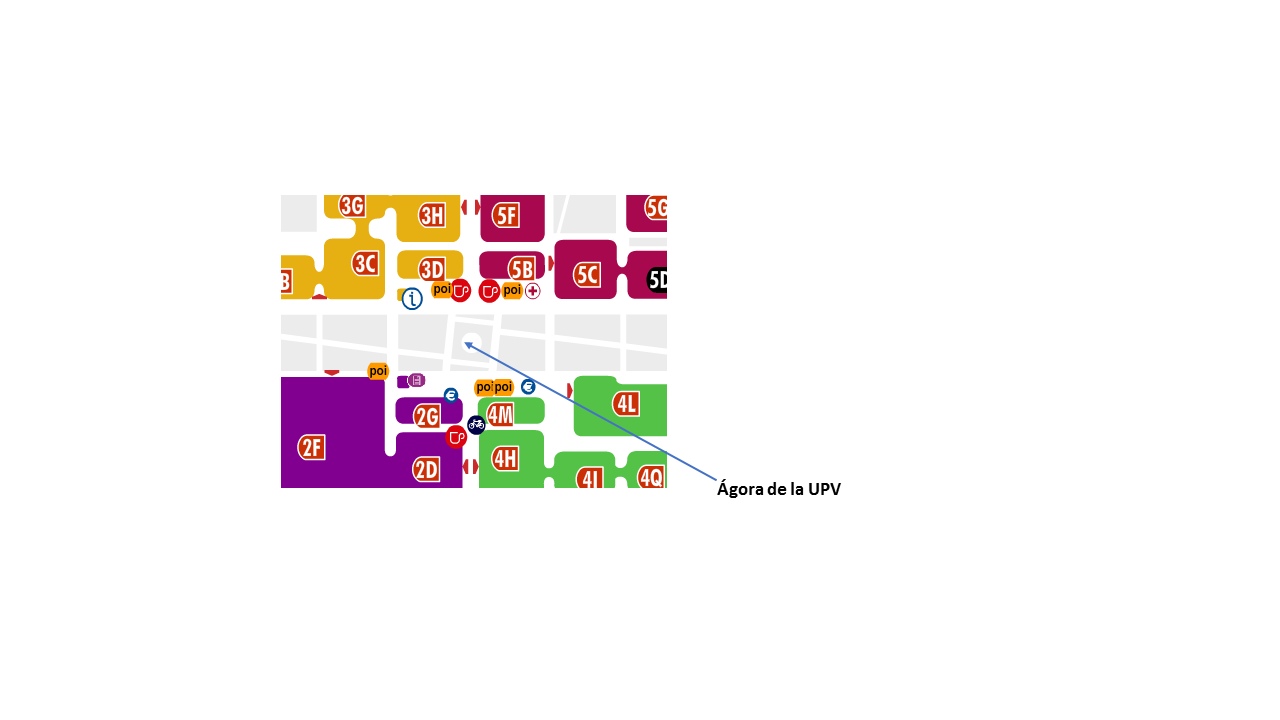
\includegraphics[trim=5cm 0cm 5cm 5cm, clip, width=1.2\textwidth]{PlanoUPV}

\end{frame}



\end{document}
